\subsection{State-Machine}\label{sec:stateMachine}

Nachdem mit dem Einleitungskapitel ein kurzer Überblick geschaffen wurde, kann nun der Hauptteil der Software genauer betrachtet werden. Der gesamte Ablauf basiert auf einer klassischen State-Machine, die aufgrund von unterschiedlichen Parametern in die entsprechenden nächsten States springt. Das hat den Vorteil, dass sich das Programm stets in einem definierten Zustand befindet und mittels entsprechenden Parametern jeweils den nächsten Arbeitsschritt vordefiniert. Die Abbildung \ref{fig:completeStateMachine} zeigt das Gesamtkonzept der State-Machine. Anschliessend werden die einzelnen States genauer definiert und beschrieben.

\begin{figure}[htbp]
	\centering
	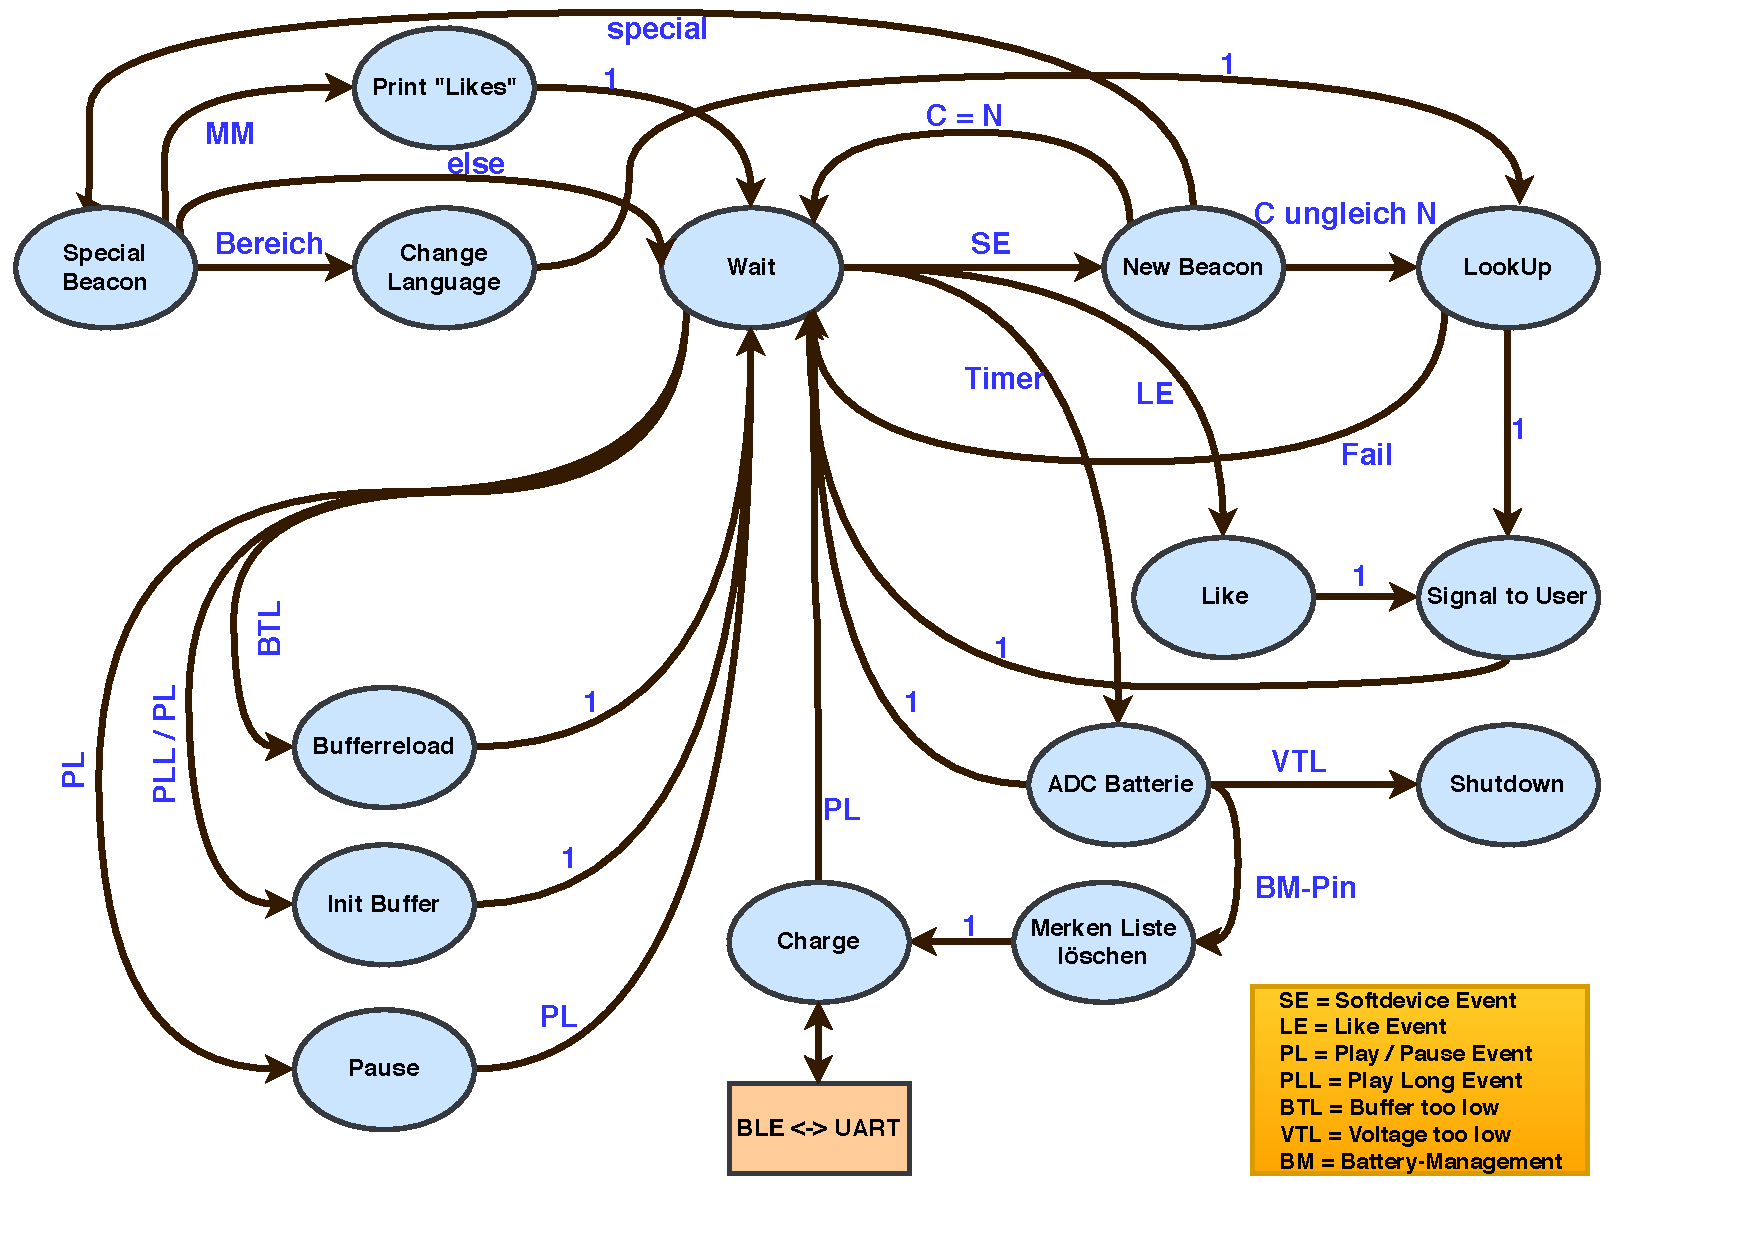
\includegraphics[width=1.01\textwidth]{Data/StateMachineFinal.pdf}
	\caption[Statemachine-Diagramm]{Statemachine im Überblick mit den einzelnen States und den Parametern}
	\label{fig:completeStateMachine}
\end{figure} 

\subsubsection*{State: Lookup}
In diesem State verschafft sich das Programm über die entsprechende Initialisierung Zugriff auf die SD-Karte der Anwendung. Falls der Mikrocontroller nicht auf die SD-Karte zugreifen kann, wird eine Fehlermeldung ausgegeben und die Funktion wird beendet. Anderenfalls wird dem Mikrocontroller signalisiert, dass der Zugriff geglückt ist und die eigentliche Funktion wird gestartet. Dazu werden die beiden Minor- und Majorzahlen in ein hexadezimales Zahlensystem gewandelt, welche dann als Vergleichskriterium verwendet werden. Falls die Nummer gefunden wird, kann das entsprechend zugehörige Audio-File über den Mikrocontroller ausgegeben werden. Verglichen wird jeweils zeilenweise, weshalb auch ein Fehlerhandling eingebaut wurde. Damit wird erkannt, ob sich das Textfile am Ende befindet. Somit lässt sich dann die Suche wiederholen, oder einen Fehler ausgeben. Die nachfolgende Abbildung \ref{fig:lookupState} zeigt den detaillierten Funktionsablauf im Lookup-State.

!!!Verknüpfung Bluetooth und Sound File!!!

\begin{figure}[htbp!!!!]
	\centering
	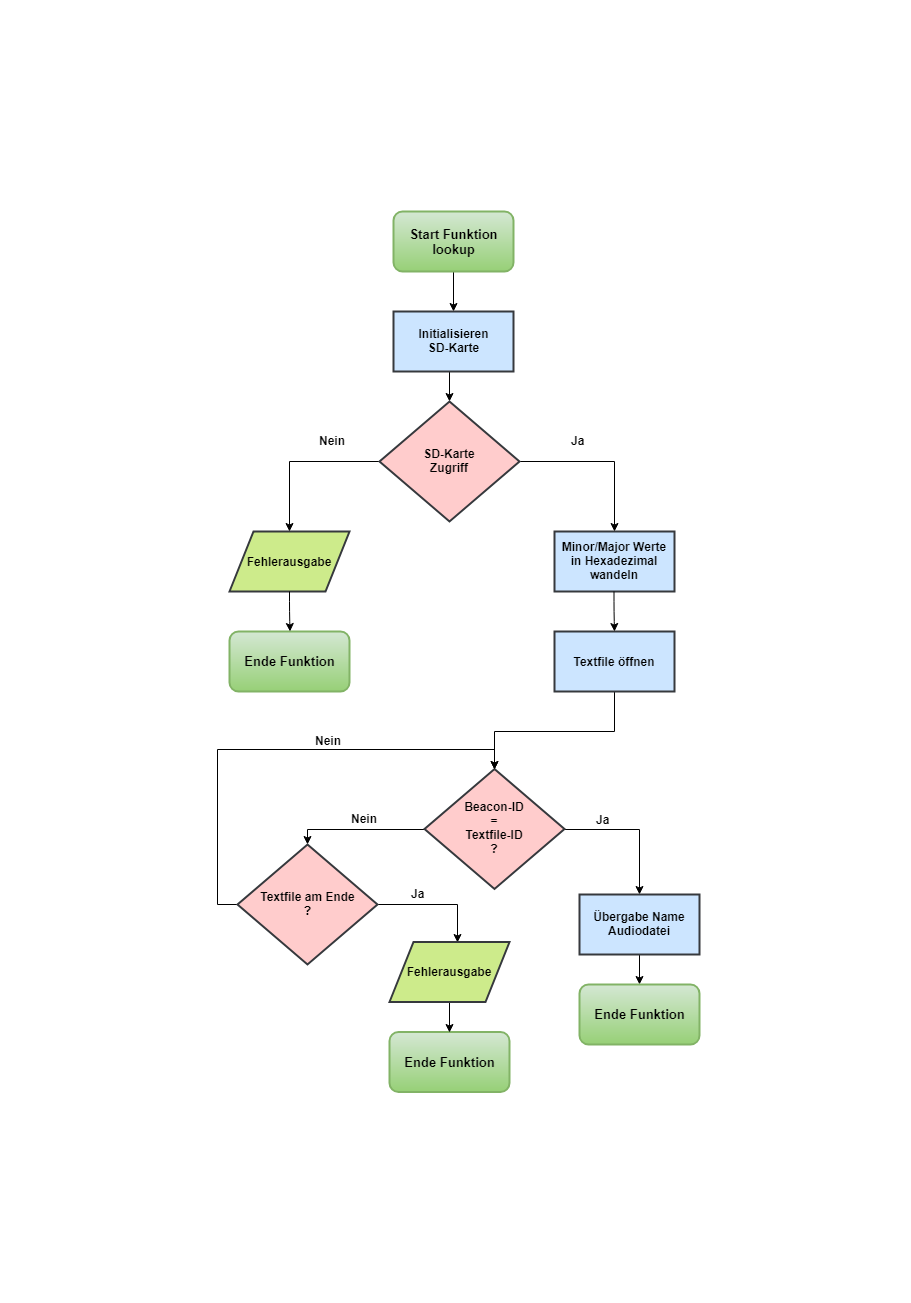
\includegraphics[width=0.57\textwidth]{Data/lookup_picture}
	\caption[Statemachine: lookup]{Funktionsablauf im lookup-State}
	\label{fig:lookupState}
\end{figure} 

\subsubsection*{State: Special Beacon}
Special Beacon dient hauptsächlich zur Unterscheidung der verschiedenen Beacons für die Sprache, das Drucken und weitere Features die in einem weiteren Ansatz implementiert werden können. Aus diesem Grund wurde dieser State auch relativ einfach gehalten. Zuerst wird verglichen, ob es sich dabei um die Sprachkonfiguration handelt. Ist dies zutreffend, so springt das Programm in den Change Language State. Anderenfalls wird überprüft, ob gerade der Like-Button gedrückt wird und entsprechend in den Print \glqq Likes \grqq State gewechselt wird. Ist keine der beiden Zustäde zutreffend, springt das Programm in den Wait State. Die nachfolgende Abbildung \ref{fig:specialBeaconState} zeigt den Ablauf der Funktion.

\begin{figure}[htbp!!!!]
	\centering
	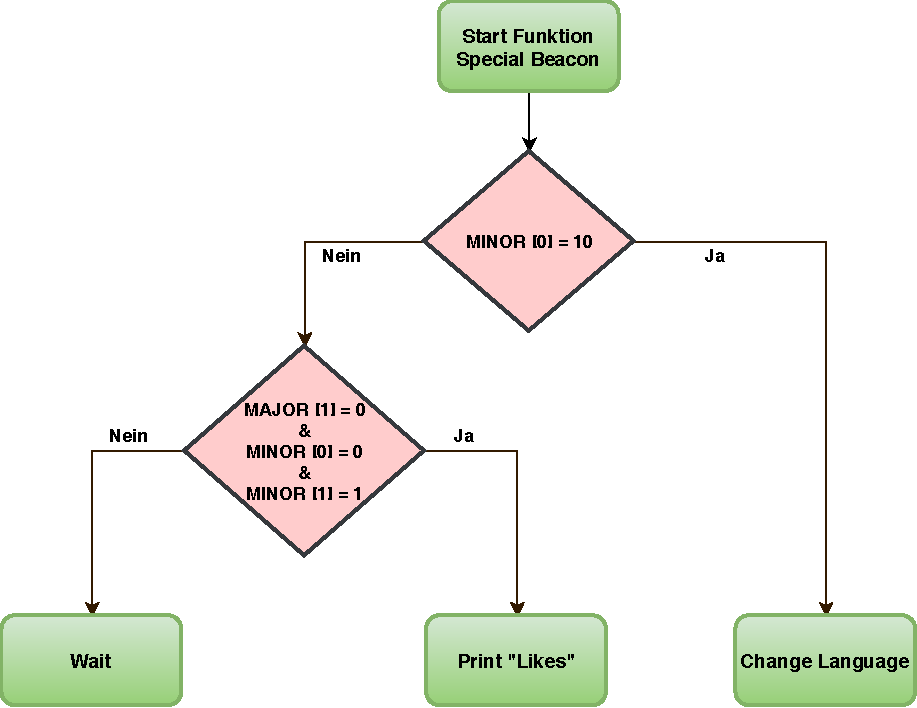
\includegraphics[width=0.9\textwidth]{Data/SpecialBeacon_picture.pdf}
	\caption[Statemachine: Special Beacon]{Funktionsablauf im Special Beacon State}
	\label{fig:specialBeaconState}
\end{figure} 
\newpage
\subsubsection*{State: Change Language}

Dieser State ist für die Sprachauswahl verantwortlich. Aufgrund des Zahlenwertes in Minor [1] wird zwischen den Landessprachen der Schweiz ausgewählt. Dabei wird die Vergleichstabelle in Form einer Datei kopiert und mit einem Kürzel entsprechend der Sprache versehen. Danach springt das Programm wieder in den lookup State.

\begin{figure}[htbp!!!!]
	\centering
	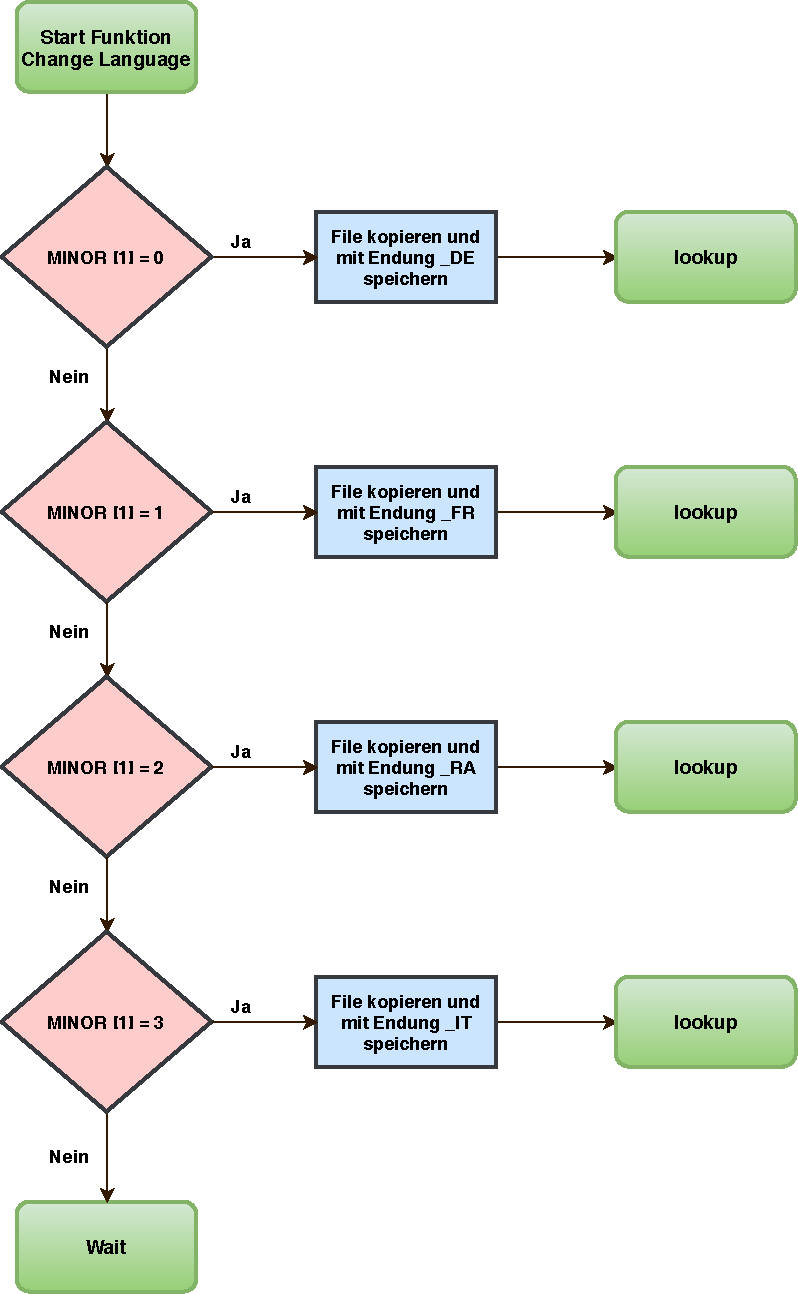
\includegraphics[width=0.7\textwidth]{Data/ChangeLanguage_picture.pdf}
	\caption[Statemachine: Change Language]{Funktionsablauf im Change Language State}
	\label{fig:changeLanguageState}
\end{figure} 

\subsubsection*{State: Print \glqq Likes\grqq}

Print \glqq Likes \grqq wurde nicht implementiert und das Hauptprogramm sprint in den Wait State. Das ist eine optionale Möglichkeit, die in einem weiteren Entwicklungskonzept bearbeitet werden kann. Die Software ermöglicht es aber diese Funktion noch einzubetten. Dabei könnte die Broschüre mit den interessanten Objekten direkt gedruckt werden und bereits für den Besucher am Ausgang des Museums bereit liegen.

\subsubsection*{State: Wait}

Dieser State ist die Ausgangslage des kompletten Ablaufs. Aufgrund von den in der Abbildung \ref{fig:waitState} ersichtlichen Bedingungen und sogenannten Flags, entscheidet das Hauptprogramm in welchen State zu switchen ist. Die Reihenfolge der Abfrage erfolgt nach dem Prioritätsprinzip.

\begin{figure}[htbp!!!!]
	\centering
	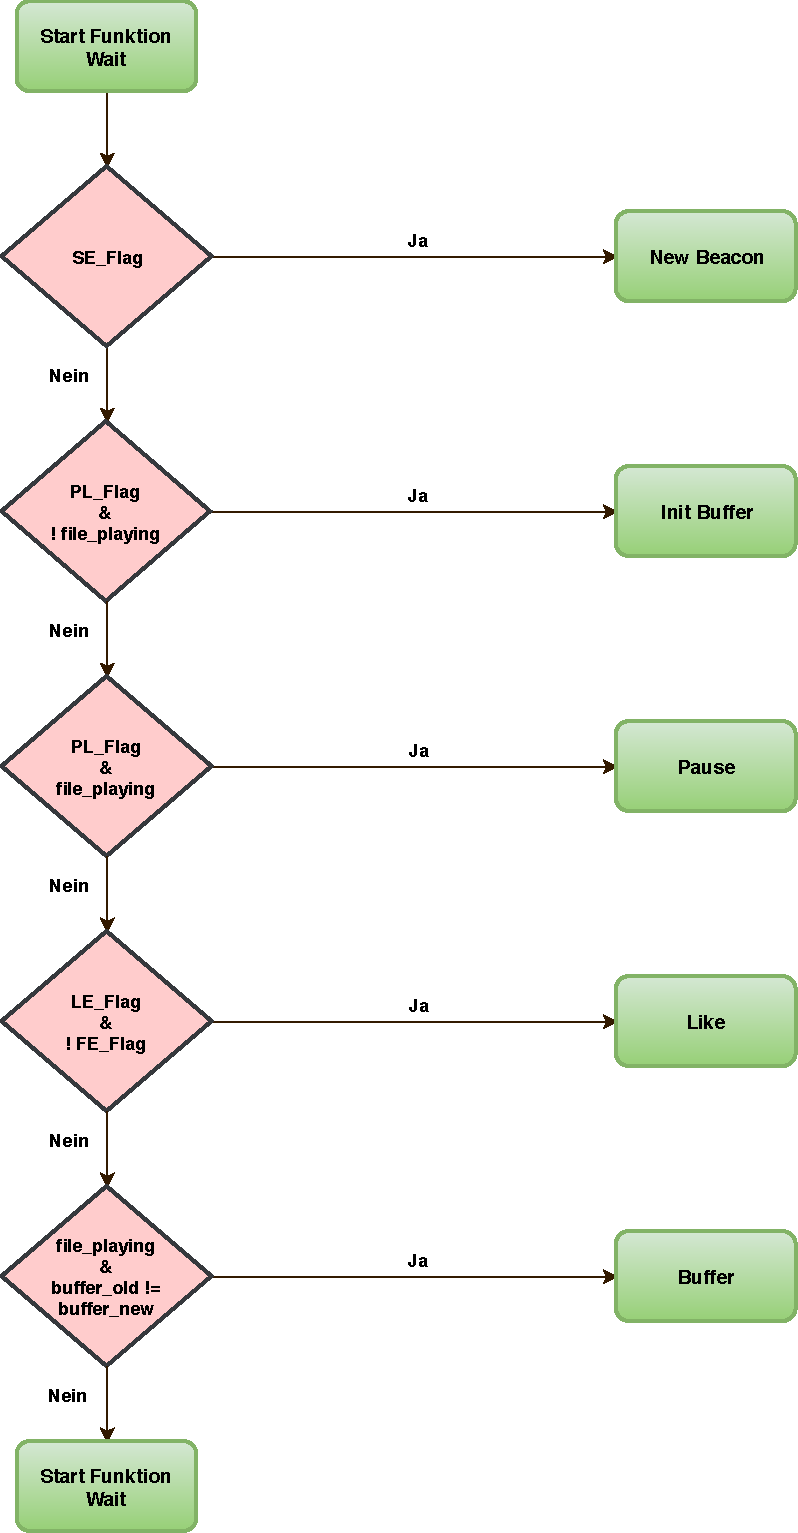
\includegraphics[width=0.7\textwidth]{Data/Wait_picture.pdf}
	\caption[Statemachine: Wait]{Funktionsablauf im Wait State}
	\label{fig:waitState}
\end{figure} 

\subsubsection*{State: New Beacon}

Wird ein Beacon erkannt, dann wird der New Beacon State aufgerufen. Ist das aktuelle Beacon immer noch das gleiche wie das alte Beacon, springt das Programm in den Wait State. Wenn es sich nicht um das gleiche Beacon handelt, wird über den lookup State überprüft, ob eine entsprechende Übereinstimmung vorhanden ist.

\begin{figure}[htbp!!!!]
	\centering
	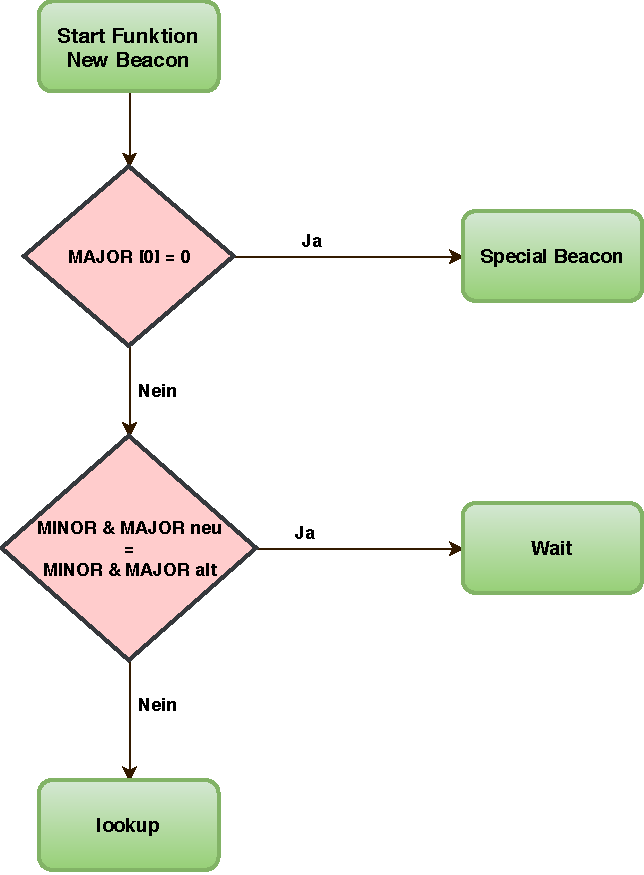
\includegraphics[width=0.5\textwidth]{Data/NewBeacon_picture.pdf}
	\caption[Statemachine: New Beacon]{Funktionsablauf im New Beacon State}
	\label{fig:newBeaconState}
\end{figure} 

\subsubsection*{State: Like}

Wird in diesem State über einen Button ein Like-Ereignis ausgelöst, springt das Programm in den Signal to User State und speichert den entsprechenden Namen des Audio-Files auf die SD-Karte. Findet kein Ereignis statt, dann wird in den Wait State gesprungen.

\subsubsection*{State: Signal to User}

Dieser State hat die Aufgabe, dem Benutzer mitzuteilen, dass ein neues Audio-File verfügbar ist, oder ob ein Kunstobjekt gespeichert wurde. Dabei blinkt eine dafür vorgesehene LED. Anschliessend springt die Software in den Wait State.

\subsubsection*{State: ADC Battery}
ADC-Battery wird zyklisch durch einen Softtimer im Wait-State aufgerufen, jedoch mit einer tiefen Priorität. Funktional wird hier die Batterie auf ihren Ladezustand überprüft und gemäss \ref{fig:adcBatteryState} entsprechend gehandelt. Wird die Batterie geladen, so wird die Like-Liste gelöscht. Anderenfalls wird das Programm in den Wait-State wechseln, oder bei ungenügendem Ladezustand das System herunterfahren.

\begin{figure}[htbp!!!!]
	\centering
	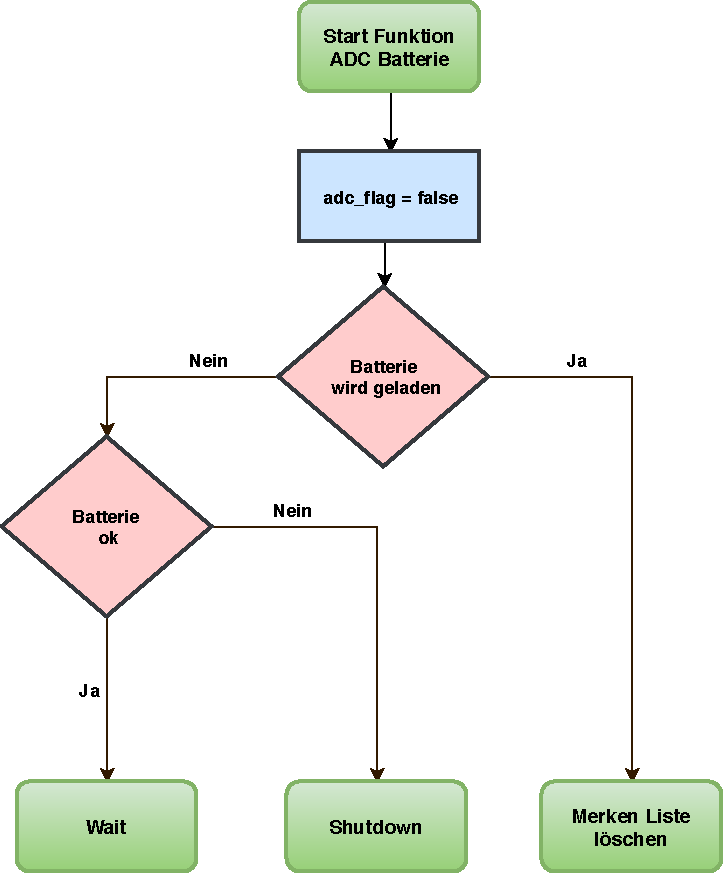
\includegraphics[width=0.5\textwidth]{Data/ADC_Battery_picture.pdf}
	\caption[Statemachine: ADC Battery]{Funktionsablauf im ADC Battery State}
	\label{fig:adcBatteryState}
\end{figure} 

\subsubsection*{State: Shutdown}

Ist der Ladezustand des Geräts zu tief, wird das System gezwungenermassen heruntergefahren. Somit sollen Schäden an der Hardware und an der Software vermieden werden.

\subsubsection*{State: Merken Liste löschen}

Dieser State löscht die Likes, um für den nächsten User bereit zu sein. Anschliessend folgt der Charge State.

\subsubsection*{State: Charge}

Hier wird überprüft, ob ein Pause- oder Playevent vorliegt. Falls ein Event vorliegt, springt die Software in den Wait-State und ist bereit für den nächsten User. Falls kein Event vorliegt, befindet sich das Programm in einer Schlaufe. Darin ist es möglich den Dojo mit der Ladestation zu verbinden und über UART Anpassungen auf der SD-Karte vorzunehmen.

\begin{figure}[htbp!!!!]
	\centering
	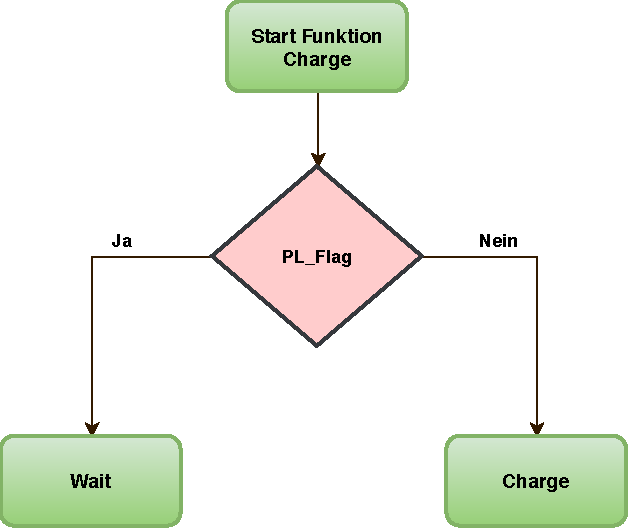
\includegraphics[width=0.5\textwidth]{Data/Charge_picture.pdf}
	\caption[Statemachine: Charge]{Funktionsablauf im Charge State}
	\label{fig:chargeState}
\end{figure} 

\subsubsection*{State: Pause}

Dieser State pausiert das Sound-File und wartet auf ein weiteres Play-Event, um die Audiodatei wieder abzuspielen.

\subsubsection*{State: Init Buffer und Bufferreload}
Diese beiden States sind für das Initialisieren des Buffers und für den Start der PWM-Funktion verantwortlich. Für weitere Informationen dazu, wird auf das Kapitel \ref{sec:sdKarte} verwiesen.